\chapter{Introdução}

A teoria de convexidade em grafos é uma área que busca adaptar os conceitos de topologia em um ambiente discreto. Naturalmente, o estudo da convexidade em grafos se estende aos grafos orientados. Dentre os vários modelos de convexidade estudados, as convexidades baseadas em caminhos, mais especificamente a convexidade \pd, onde um vértice é gerado por um conjunto se possui vizinhança de entrada e vizinhança de saída neste conjunto, introduzida em~\cite{ERDOS1972}, será o foco deste trabalho.

Para introduzir os conceitos básicos de convexidade em grafos, iremos revisitar os conceitos básicos da \emph{geometria convexa}. Para uma leitura um pouco mais detalhada, vale checar o capítulo inicial de~\cite{julio}. Seja $d$ um inteiro tal que $d \geq 2$ e $\mathbb{R}^d$ o espaço (euclidiano) $d$-dimensional, um determinado conjunto $S \subseteq \mathbb{R}^d$ é convexo se para qualquer segmento de reta entre dois pontos de $S$, o mesmo está contido em $S$.

\begin{figure}[ht]
    \centering
    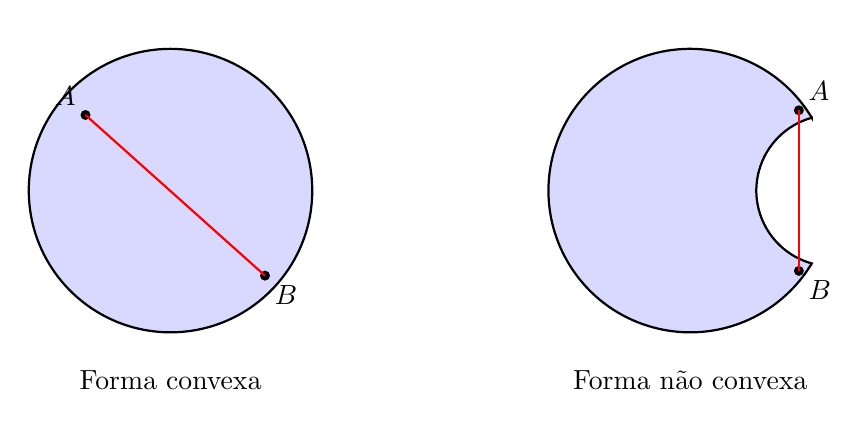
\begin{tikzpicture}[scale=1.2]
    \begin{scope}
        \draw[thick, fill=blue!15] (0,0) circle (1.5);
        \fill (-0.9,0.8) circle (1.5pt) node[above left] {$A$};
        \fill (1.0,-0.9) circle (1.5pt) node[below right] {$B$};
        \draw[thick, red] (-0.9,0.8) -- (1.0,-0.9);
        \node at (0,-2) {Forma convexa};
    \end{scope}
    \begin{scope}[xshift=5.5cm]
        \path[fill=blue!15, draw=black, thick]
        (30.93:1.5) arc (30.93:329.07:1.5)
        arc (254.54:105.46:0.8) -- cycle;
        \fill (1.15,0.85) circle (1.5pt) node[above right] {$A$};
        \fill (1.15,-0.85) circle (1.5pt) node[below right] {$B$};
        \draw[thick, red] (1.15,0.85) -- (1.15,-0.85);
        \node at (0,-2) {Forma não convexa};
    \end{scope}
  
\end{tikzpicture}
\caption{Representação de uma forma convexa (esquerda) e uma forma não convexa (direita)}
\end{figure}

Seja $A$ um conjunto não vazio, uma convexidade $\mathcal{C}$, é uma família de subconjuntos de $A$, tal que:

\begin{enumerate}
    \item $\emptyset, A \in \mathcal{C}$
    \item $\mathcal{C}$ é fechado sob interseção
    \item A união infinita de conjuntos conexos aninhados, é convexa
\end{enumerate}

Observe que quando o conjunto $V$ é finito, como por exemplo o conjunto de vértices de um grafo, a propriedade $3$ pode ser descartada. Seja $C \in \mathcal{C}$, $C$ é um conjunto convexo. Seja $V$ um conjunto finito e não vazio e $\mathcal{C}$ uma convexidade sobre o mesmo. Seja $S \subseteq V$, a \emph{evoltória convexa} de $S$, denotada por $conv(S)$, é o menor conjunto convexo que contém $S$. Para todo $S, S' \subseteq V$, $conv(S)$ tem as seguintes propriedades que o definem com \emph{operador de fecho}:

\begin{enumerate}
    \item $S \subseteq conv(S)$ (extensividade)
    \item $S \subseteq S' \implies conv(S) \subseteq conv(S')$ (monotonicidade)
    \item $conv(\emptyset) = \emptyset$ (normalização)
    \item $conv(conv(S)) = conv(S)$ (idempotência)
\end{enumerate}

Seja $S \subseteq V$ e que o mesmo é convexo em $\mathcal{C}$ e seja $x \in S$, dizemos que $x$ é um \emph{ponto extremo} ou \emph{vértice extremo} de $S$, se $x \notin conv(S\backslash \{x\})$, denotamos com \ext{S}, o conjunto de vértice extremos de $S$.

Seja I:~$2^V \longrightarrow 2^V$, dizemos que I é uma \emph{função de intervalo} sobre $V$ se para todo $S, S' \subseteq V$:

\begin{enumerate}
    \item $S \subseteq \text{I}(S)$ (extensividade)
    \item $S \subseteq S' \implies \text{I}(S) \subseteq \text{I}(S')$ (monotonicidade)
    \item I$(\emptyset) = \emptyset$ (normalização)
\end{enumerate}

Dizemos que uma função de intervalo I$(\cdot)$ sobre $V$ \emph{induz} a família de conjuntos $S\subseteq V$ tal que I$(S) = S$. Em~\cite{calder1971}, vemos uma definição semelhante a essa apresentada. Além disso, em~\cite{calder1971} e~\cite{vandevel1993}, vemos que essa família de conjuntos induzida por I$(\cdot)$ é uma convexidade. Neste caso, toda função de intervalo induz uma única convexidade, mas toda convexidade pode ser induzida por uma ou mais funções de intervalo. Uma convexidade $\mathcal{C}$ definida por uma função de intervalo, é chamada de \emph{convexidade de intervalo}, veremos alguns exemplos posteriormente.

Temos que o fecho convexo de um conjunto $S$, pode ser obtido por meio da aplicação sucessiva da função de intervalo I$(S)$, com isso temos que:

\[
conv(S) = \bigcup_{k=1}^{\infty}\text{I}^k(S)
\]

Perceba que o indice $k$ indica a $k$-ésima iteração da função de intervalo, em grafos teriamos que $k \leq n$, onde $n$ é o número de vértices. Também dizemos que o \emph{tempo de iteração} de um subconjunto $S\subseteq V$ é o menor inteiro $k$, tal que $\text{I}^k(S) = conv(S)$.

\section{Convexidade em grafos (orientados)}

% Seja $D$ um grafo finito orientado e $V(D)$ o conjunto de vértices do mesmo. $\mathcal{C}$ é uma \emph{convexidade} no grafo $D$ se $\mathcal{C}$ é uma convexidade de intervalos sobre $V(D)$. Seja $S \subseteq V(D)$ um conjunto de envoltória mínimo de $D$, o temos que $|S|$ é denominado como \emph{número de envoltória} e denotado por $hn(D)$. Seja $S \subseteq V(D)$, se I$(S) = V(D)$, temos que $S$ é um \emph{conjunto de intervalo}, o \emph{número de intervalo}, denotado por $in(D)$ é a cardinalidade de um conjunto de intervalo mínimo em $D$.

A teoria da convexidade em grafos é uma área que busca adaptar os conceitos de topologia e geometria contínua em um ambiente discreto, um dos primeiros trabalhos a abordar formalmente o tema foi \textit{Convexity in Graphs}~\cite{harary1981}. Naturalmente, o estudo da convexidade se estende aos grafos orientados. Dentre os vários tipos de convexidade estudados, temos as convexidades baseadas em caminhos, como por exemplo a \emph{convexidade de caminhos de tamanho 2}, introduzido em~\cite{CENTENO200911}, denotado por $P_3$, onde um vértice é gerado por um conjunto $S \subseteq V(G)$ se possui dois vizinhos em $S$, ou a \emph{convexidade geodésica}, onde dado dois vértices $u,v \in S \subseteq V(G)$, todos os vértices que pertencem ao menor $(u,v)$-caminho são gerados, introduzido em\cite{HARARY199389}.

No contexto de grafos orientados, temos por exemplo as versões das convexidades apresentadas anteriormente, como a convexidade $\overrightarrow{P_3}$, onde um vértice é gerado por um conjunto se possui vizinhança de entrada e vizinhança de saída neste conjunto, introduzida em~\cite{ERDOS1972} ou a \emph{convexidade geodésica} orientada, onde dados dois vértices $u,v \in S \subseteq V(D)$, todos os vértices no menor $u,v$-caminho ou $v,u$-caminho são gerados.

Essas operações descritas para gerar novos vértices é o que chamamos anteriormente de \emph{funções de intervalo}, e que neste trabalho, as funções de intervalo são baseadas em caminhos nos grafos. Dado um subconjunto inicial de vértices $S$, aplicamos a função de intervalo nesse conjunto para gerar novos vértices. Traduzindo para grafos, dizemos que um subconjunto $S \subseteq V(D)$ é \emph{convexo} se, para qualquer $u,v \in S$, $I(u,v) \in S$. O \emph{fecho convexo}, denotado por $conv(S)$, é o menor conjunto convexo que contém $S$. Se $conv(S) = V(D)$, dizemos que $S$ é um conjunto de envoltória.

Com base nessas definições, podemos definir alguns parâmetros que são bastante estudados em diversas convexidades. O \emph{número de envoltória}, denotado por $hn(D)$ é o tamanho do menor conjunto de envoltória em $D$. Denotamos o número de envoltória orientado como $\overrightarrow{hn}(D)$. O \emph{tempo de iteração} de um conjunto $S \subseteq V(D)$, denotado por $ti(S)$, é basicamente a quantidade de vezes que é necessário aplicar uma função de intervalo até obter o fecho convexo $conv(S)$.

\begin{figure}[ht]
    \centering
    \begin{subfigure}[t]{0.48\textwidth}
        \centering
        \begin{tikzpicture}[scale=.6,
            vertex/.style={circle, draw, thick, minimum size=0.9cm, font=\normalsize},
            arco/.style={-{Latex[length=2mm, width=2.4mm]}, line width=1.1pt},
            branco/.style={fill=white},
            cinza/.style={fill=gray!40, draw=gray!70!black},
            azul/.style={fill=blue!20, draw=blue!60!black},
            vermelho/.style={fill=red!30, draw=red!70!black}
        ]
            \node[vertex, cinza] (v1) at (0, 2) {$v_1$};
            \node[vertex, cinza] (v2) at (0, 0) {$v_2$};
            \node[vertex, branco] (v3) at (2.2, 1) {$v_3$};
            \node[vertex, branco] (v4) at (4.4, 0) {$v_4$};
            \node[vertex, branco] (v5) at (4.4, 2) {$v_5$};
            \node[vertex, branco] (v6) at (6.6, 1) {$v_6$};

            \draw[arco] (v1) -- (v3);
            \draw[arco] (v3) -- (v2);
            \draw[arco] (v4) -- (v2);
            \draw[arco] (v3) -- (v4);
            \draw[arco] (v1) -- (v5);
            \draw[arco] (v5) -- (v3);
            \draw[arco] (v6) -- (v4);
            \draw[arco] (v5) -- (v6);
        \end{tikzpicture}
        \caption{Etapa 0: conjunto inicial $S=\{v_1,v_2\}$.}\label{fig:inf-a}
    \end{subfigure}
    \hfill
    \begin{subfigure}[t]{0.48\textwidth}
        \centering
        \begin{tikzpicture}[scale=.6,
            vertex/.style={circle, draw, thick, minimum size=0.9cm, font=\normalsize},
            arco/.style={-{Latex[length=2mm, width=2.4mm]}, line width=1.1pt},
            branco/.style={fill=white},
            cinza/.style={fill=gray!40, draw=gray!70!black},
            azul/.style={fill=blue!20, draw=blue!60!black},
            vermelho/.style={fill=red!30, draw=red!70!black}
        ]
            \node[vertex, cinza] (v1) at (0, 2) {$v_1$};
            \node[vertex, cinza] (v2) at (0, 0) {$v_2$};
            \node[vertex, vermelho] (v3) at (2.2, 1) {$v_3$};
            \node[vertex, branco] (v4) at (4.4, 0) {$v_4$};
            \node[vertex, branco] (v5) at (4.4, 2) {$v_5$};
            \node[vertex, branco] (v6) at (6.6, 1) {$v_6$};
            \draw[arco] (v1) -- (v3);
            \draw[arco] (v3) -- (v2);
            \draw[arco] (v4) -- (v2);
            \draw[arco] (v3) -- (v4);
            \draw[arco] (v1) -- (v5);
            \draw[arco] (v5) -- (v3);
            \draw[arco] (v6) -- (v4);
            \draw[arco] (v5) -- (v6);


        \end{tikzpicture}
        \caption{Etapa 1: $v_3$ é infectado por $v_1$ e $v_2$.}\label{fig:inf-b}
    \end{subfigure}

    \vspace{1.5em}

    \begin{subfigure}[t]{0.48\textwidth}
        \centering
        \begin{tikzpicture}[scale=.6,
            vertex/.style={circle, draw, thick, minimum size=0.9cm, font=\normalsize},
            arco/.style={-{Latex[length=2mm, width=2.4mm]}, line width=1.1pt},
            branco/.style={fill=white},
            cinza/.style={fill=gray!40, draw=gray!70!black},
            azul/.style={fill=blue!20, draw=blue!60!black},
            vermelho/.style={fill=red!30, draw=red!70!black}
        ]
            \node[vertex, cinza] (v1) at (0, 2) {$v_1$};
            \node[vertex, cinza] (v2) at (0, 0) {$v_2$};
            \node[vertex, azul] (v3) at (2.2, 1) {$v_3$};
            \node[vertex, vermelho] (v4) at (4.4, 0) {$v_4$};
            \node[vertex, vermelho] (v5) at (4.4, 2) {$v_5$};
            \node[vertex, branco] (v6) at (6.6, 1) {$v_6$};
            \draw[arco] (v1) -- (v3);
            \draw[arco] (v3) -- (v2);
            \draw[arco] (v4) -- (v2);
            \draw[arco] (v3) -- (v4);
            \draw[arco] (v1) -- (v5);
            \draw[arco] (v5) -- (v3);
            \draw[arco] (v6) -- (v4);
            \draw[arco] (v5) -- (v6);

        \end{tikzpicture}
        \caption{Etapa 2: $v_4$ é infectado pelos vértices $v_2$ e $v_3$ e o vértice $v_5$ é infectado pelos vértices $v_1$ e $v_3$.}\label{fig:inf-c}
    \end{subfigure}
    \hfill
    \begin{subfigure}[t]{0.48\textwidth}
        \centering
        \begin{tikzpicture}[scale=.6,
            vertex/.style={circle, draw, thick, minimum size=0.9cm, font=\normalsize},
            arco/.style={-{Latex[length=2mm, width=2.4mm]}, line width=1.1pt},
            branco/.style={fill=white},
            cinza/.style={fill=gray!40, draw=gray!70!black},
            azul/.style={fill=blue!20, draw=blue!60!black},
            vermelho/.style={fill=red!30, draw=red!70!black}
        ]
            \node[vertex, cinza] (v1) at (0, 2) {$v_1$};
            \node[vertex, cinza] (v2) at (0, 0) {$v_2$};
            \node[vertex, azul] (v3) at (2.2, 1) {$v_3$};
            \node[vertex, azul] (v4) at (4.4, 0) {$v_4$};
            \node[vertex, azul] (v5) at (4.4, 2) {$v_5$};
            \node[vertex, vermelho] (v6) at (6.6, 1) {$v_6$};
            \draw[arco] (v1) -- (v3);
            \draw[arco] (v3) -- (v2);
            \draw[arco] (v4) -- (v2);
            \draw[arco] (v3) -- (v4);
            \draw[arco] (v1) -- (v5);
            \draw[arco] (v5) -- (v3);
            \draw[arco] (v6) -- (v4);
            \draw[arco] (v5) -- (v6);

        \end{tikzpicture}
        \caption{Etapa 3: $v_6$ é infectado pelos vértices $v_4$ e $v_5$. Todo o grafo está infectado.}\label{fig:inf-d}
    \end{subfigure}

    \caption{Processo de infecção na convexidade $P_3$ direcionada}\label{fig:convexidade-p3-processo}
\end{figure}

Se dado um subconjunto $S \subseteq V(D)$, $I(S) = V(D)$ em um única iteração, temos que $S$ é um \emph{conjunto de intervalo}. Com isso, temos um outro parâmetro bastante estudado em convexidade, o \emph{número de intervalo}, denotado por $in(D)$, que é basicamente o tamanho do menor conjunto de intervalo em $D$. Denotamos o número de intervalo orientado como $\overrightarrow{in}(D)$.

\begin{figure}[ht]
    \centering
	\begin{tikzpicture}[scale=.6,
            vertex/.style={circle, draw, minimum size=0.8cm, font=\small},
            branco/.style={fill=white},
	    arco/.style={-{Latex[length=2mm, width=2.4mm]}, line width=1.1pt},
            vermelho/.style={fill=red!30, draw=red!70!black},
            cinza/.style={fill=gray!40, draw=gray!70!black}
        ]

	\node[vertex, cinza] (v1) at (2.5, 3)  {$v_1$};
        \node[vertex, branco]   (v2) at (0,   1.5){$v_2$};
        \node[vertex, branco]   (v3) at (5,   1.5){$v_3$};
        \node[vertex, cinza] (v4) at (1,   0)  {$v_4$};
        \node[vertex, cinza] (v5) at (4,   0)  {$v_5$};
        \node[vertex, cinza] (v6) at (8,   0)  {$v_6$};
        \node[vertex, branco]   (v7) at (10,  1.5){$v_7$};
        \node[vertex, cinza] (v8) at (8,   3)  {$v_8$};

        \draw[arco] (v1) -- (v2);
        \draw[arco] (v1) -- (v3);
        \draw[arco] (v1) -- (v4);
        \draw[arco] (v2) -- (v3);
        \draw[arco] (v2) -- (v4);
        \draw[arco] (v3) -- (v5);
        \draw[arco] (v1) -- (v8);
        \draw[arco] (v3) -- (v8);
        \draw[arco] (v8) -- (v6);
        \draw[arco] (v3) -- (v7);
        \draw[arco] (v7) -- (v8);
        \draw[arco] (v6) -- (v7);
    \end{tikzpicture}
    \caption{Os vértices em cinza formam um conjunto de intervalo com cardinalidade 5.}\label{fig:convexidade-p3}
\end{figure}

\section{Espectro}\label{espectro-basico}

Dado um grafo $G$ e um parâmetro de convexidade, o \emph{espectro} de um determinado parâmetro é o conjunto de valores que o parâmetro assume em todas as possíveis orientações de $G$, denotado por $S_c$, onde $c$ é uma convexidade de sua escolha, por exemplo, $S_g$ é o espectro \emph{geodésico}. Formalmente o conceito de espectro foi introduzido na convexidade geodésica em \textit{Geodetic Spectra of graphs}~\cite{CHANG2004}, em que o parâmetro estudado foi o \emph{número de intervalo} que também é chamado de \emph{número geodésico}, também foi introduzido o conceito de \emph{espectro geodésico forte}, em que temos apenas orientações fortes do grafo $G$, vale ressaltar que um grafo $G$ tem orientações fortes se e somente se não tem pontes e é conexo.

Dizemos que o espectro é \emph{contínuo} se o mesmo assume todos os valores inteiros no intervalo entre o limite inferior e o limite superior.

\section{Contribuições e Organização do texto}


